\chapter{Projetos de novas instalações produtivas (localização, capacidade e rede de operações)} 
\label{chap:projetos_de_novas} 

\section{Cadeia de suprimentos: estrutura, verticalização e terceirização} 
\label{sec:projetos_de_novas_supply_chain} 
A cadeia de suprimentos de um processo produtivo é a relação da empresa com seus fornecedores e clientes, e a relação destes com seus fornecedores e clientes como descrita na Figura \ref{fig:supply_chain}. Nesta figura é possível perceber que os fornecedores que lidam diretamente com a operação são os de primeira camada, e os fornecedores dos fornecedores compõem a segunda camada, e estes fazem parte da montante do processo. Igualmente para o lado jusante, que tem os clientes de primeira camada, contato direto com a operação, e clientes dos clientes, que são os de segunda camada.
\par Além disso nota-se que fornecedores e clientes de primeira camada fazem parte da rede imediata de fornecimento, e a rede completa é chamada de rede total de suprimentos.


\begin{figure}[H]
    \centering
    \caption{Cadeia de Suprimentos (supply chain)}
    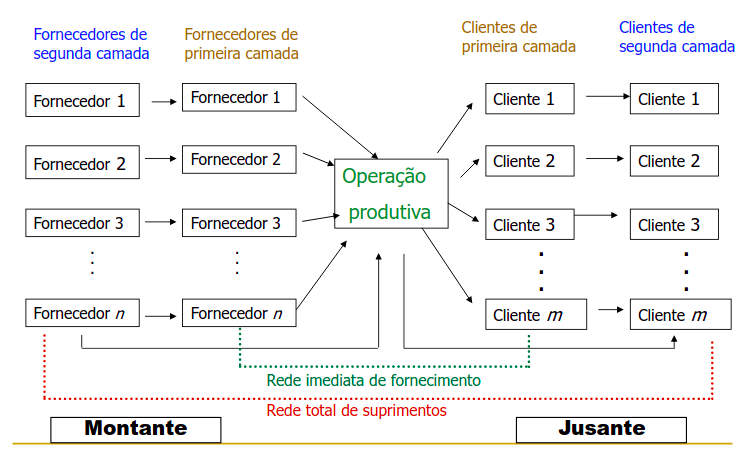
\includegraphics[width =\textwidth]{images/supply_chain.png}
    \caption*{Fonte: \cite{supplychain}}
    \label{fig:supply_chain}
\end{figure}
  
\par A importância de entender toda a rede é vital para a competitividade da empresa devido aos seguintes aspectos: identificar a relações imediatas, isso ajuda a conhecer melhor fornecedores e clientes; identificar elos significativos, saber quais partes da rede contribuem para alcançar os objetivos de desempenho valorizados pelos clientes finais, esta análise começa primeiramente pela parte da jusante e depois pela montante da rede a partir dos quais mais contribuem para o serviço do consumidor final, e por último, focar em questões de longo prazo, alguns elos dessa rede podem gerar situações como greves ou parada de máquina que ocasione uma interrupção no fluxo da operação, é importante estudar a possibilidade de ajudar ou substituir esse elo mais fraco.

\section{A capacidade adequada de uma instalação industrial}
A demanda de produção que será atendida pela fábrica depende de dois fatores: a demanda disponível no mercado e em segundo lugar, o capital disponível para investimento. 

Para se reduzir os custos de produção a ponto de gerar uma economia de escala, é recomendado que a produção esteja sempre aproveitando a sua capacidade total. Esta prática confere vantagens como o aumento da participação da empresa no mercado, maximização das vendas, beneficio com os menores custos unitários. Entende-se como "Custo unitário de produção"  o custo para se produzir uma unidade do produto, gerado pela divisão do custo total de produção de um lote pelo número de unidades do lote.

Na prática, este habito citado não possui exatamente o efeito esperado. O uso constante da capacidade maxima da fabrica gera stress nos equipamentos e trabalhadores e isto certamente causa aumentos inesperados nos custos de produção.

Conclue-se que a capacidade instalada de uma nova unidade de produção deve ser definida pelo seu "projeto da capacidade", porém, a sua capacidade real é posteriormente calculada em meio a operação da fábrica, comparando seus custos com todos os volumes possíveis de produção. 

\section{Verticalização x Terceirização}
É chamada de Verticalização, a estratégia que prevê a produção interna dos recursos que serão usados na fabricação de um produto ou na prestação de um serviço. Usando esta tática de gestão, toda a produção estará sob a inteira responsabilidade da própria empresa.

Por outro lado, nenhuma empresa faz tudo que é necessário para fabricar seus produtos sozinha. A forma de organização estrutural que permite a uma empresa transferir a outra suas atividades é chamada de Terceirização. Esta forma proporciona maior disponibilidade de recursos para sua atividade-fim, reduz a estrutura operacional, diminui custos, economiza recursos e desburocratiza a administração.

\par O suprimento interno ou terceirizado pode afetar diretamente os objetivos de desempenho de uma operação, sendo assim, cada estratégia oferece um pacote de vantagens e desvantagens, o que torna a decisão mais complexa e importante. Antes da escolha, é necessário sempre observar a importância estratégica da atividade. 


\section{Aplicação Prática} 
\label{sec:projetos_de_novas_aplicacao}
Para a SunBurn a escolha da localização onde seus parques de energia solar seriam implantados foi escolhida conforme os dois fatores fundamentais para esse tipo de sistema produtivo: um grande espaço e estudo prévio durante dois anos para verificar o índice de irradiação solar naquele local. 
\par Por esses motivos a reunião Nordeste foi escolhida para implementar os parques solares, já que esta dispõe dos dois elementos fundamentais.

\par A cadeia de suprimentos da SunBurn encontra-se descrita na Figura \ref{fig:cadeia_suprimentos_sunburn}. Nesta figura encontram-se definidas as relações da montante (fornecedores) e da jusante (cliente) com a operação produtiva. Também são identificados os fornecedores fixos e os sob cotação e demanda, além dos fluxos de serviço e de informação que existe entre cada elemento deste fluxograma. 


\begin{figure}[H]
    \centering
    \caption{Cadeia de Suprimentos da SunBurn.}
    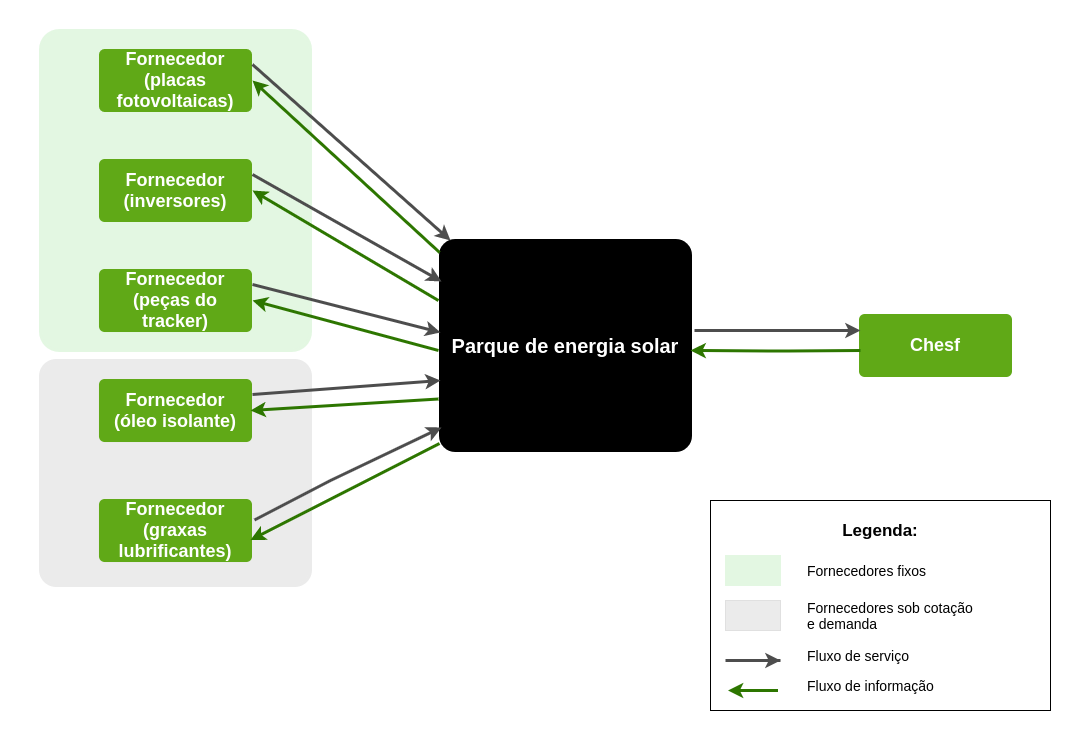
\includegraphics[width = \textwidth]{images/cadeia_suprimentos_sunburn.png}
    \caption*{Fonte: Autoria própria.}
    \label{fig:cadeia_suprimentos_sunburn}
\end{figure}
  

